\chapter{Lecture 7 - Introduction to Linear Algebra and Gauss Elimination}
\label{ch:lec7n}
\section{Objectives}
The objectives of this lecture are to:
\begin{itemize}
\item Provide background and describe why engineers what to solve systems of linear equations.
\item Describe and demonstrate the Gauss elimination algorithm.
\item Do an example in MATLAB.
\end{itemize}
\setcounter{lstannotation}{0}

\section{Background}

Linear systems of equations arise in a variety of contexts.  For example, consider a simple analysis of a truss structure as shown in Figure \ref{fig:lec7n-truss}.  If you are to conduct a simple static analysis of this structure, you would need to derive equilibrium equations to show that the sum of forces at each point---A, B, C, D, E, and F---in the $x$- and $y$-direction equals zero.  A total of eight equations are drived in this way and shown below.
\begin{marginfigure}
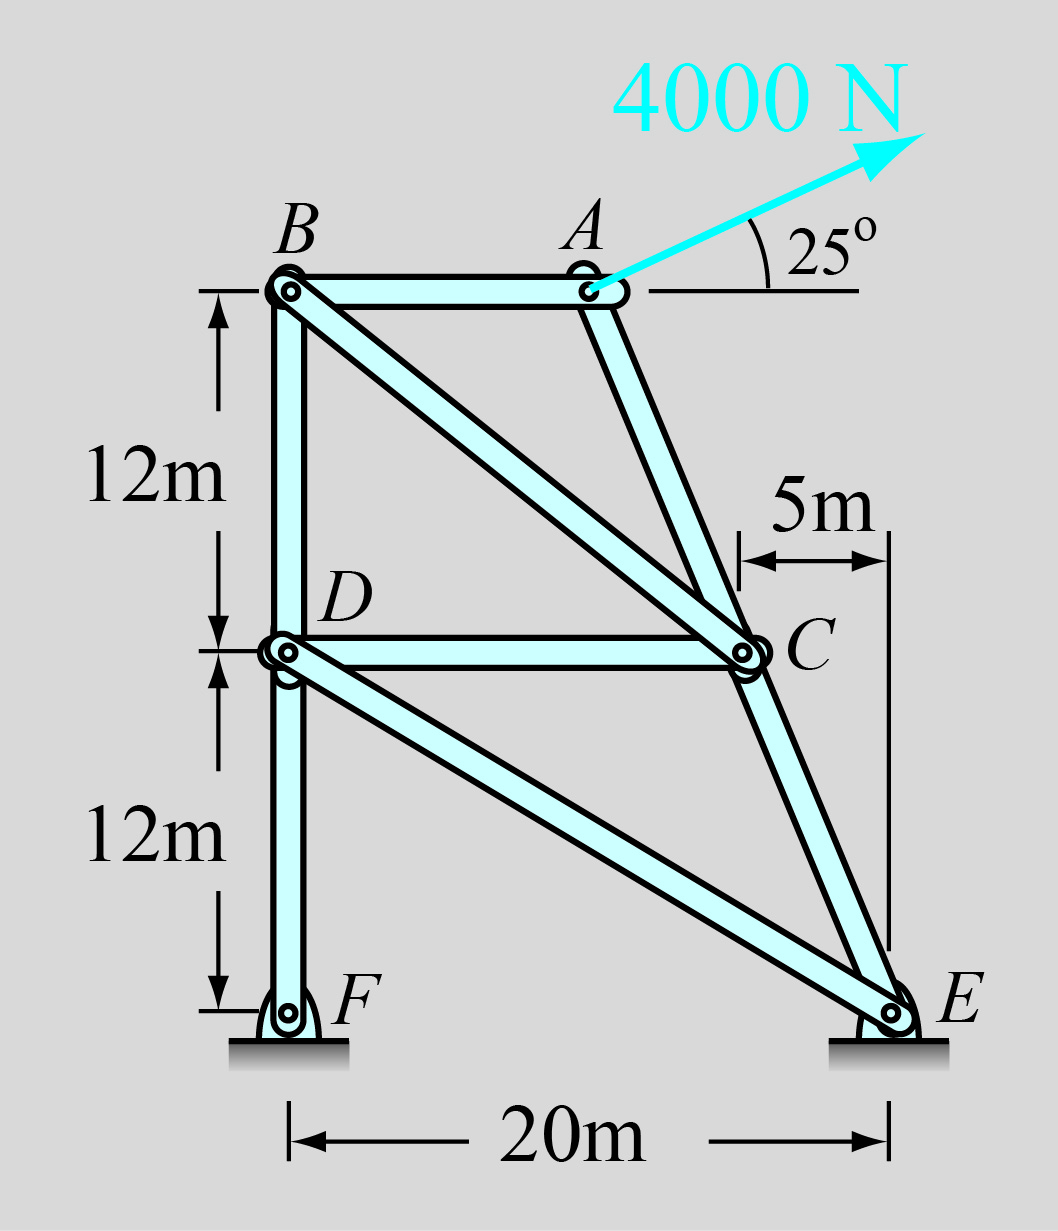
\includegraphics{Chapter4Example4_3.jpg}
\caption{Two-dimensional truss structure.}
\label{fig:lec7n-truss}
\end{marginfigure}
%\begin{fullwidth}
\begin{centering}
\begin{table}
\begin{tabular}{l l l}
$-F_{AB} - 0.3846F_{AC} = 3625$ & $0.9231F_{AC} = 1690$ & $\sum F_{x}$, $\sum {F_y}$ at A \\
$F_{AB} - 0.7809 F_{BC}=0$ & $0.6247F_{BC} - F_{BD} = 0$ & $\sum F_{x}$, $\sum {F_y}$ at B\\
\multicolumn{2}{l}{$- 0.3846F_{AC} - 0.7809F_{BC} - F_{CD} + 0.3846F_{CE}  = 0$} & $\sum F_{x}$ at C \\
\multicolumn{2}{l}{$0.9231F_{AC}+0.6247F_{BC} - 0.9231F_{CE} = 0$} & $\sum F_{y}$ at C \\
$F_{CD}+0.8575F_{DE} = 0$ & $F_{BD} - 0.5145F_{DE} - F_{DF} = 0$ & $\sum F_{x}$, $\sum {F_y}$ at D\\
\end{tabular}
\end{table}
\end{centering}
%\end{fullwidth}
We cannot, in general, solve these equations individually, the unknown values---the tension in each of the eight truss elements---are distributed among all of the equations.  In general we must solve the equations simultaneously; the resulting linear equations are shown in matrix-vector form in Equation \ref{eq:lec7n-truss-soe}.
\begin{fullwidth}
\begin{equation}
\left[
\begin{matrix}
-1 & -0.3846 & 0 & 0 & 0 & 0 & 0 & 0 \\
0 & 0.9231 & 0 & 0 & 0 & 0 & 0 & 0 \\
1 & 0 & -0.7809 & 0 & 0 & 0 & 0 & 0 \\
0 & 0 & 0.6247 & -1 & 0 & 0 & 0 & 0 \\
0 & -0.3846 & -0.7809 & 0 & -1 & 0.3846 & 0 & 0 \\
0 & 0.9231 & 0.6247 & 0 & 0 & -0.9231 & 0 & 0 \\ 
0 & 0 & 0 & 0 & 1 & 0 & 0.8575 & 0 \\
0 & 0 & 0 & 1 & 0 & 0 & -0.5145 & - 1 \\
\end{matrix}
\right]
\left[
\begin{matrix}
F_{AB} \\
F_{AC} \\
F_{BC} \\
F_{BD} \\
F_{CD} \\
F_{CE} \\
F_{DE} \\
F_{DF} 
\end{matrix}
\right]
=
\left[
\begin{matrix}
3625 \\
1690 \\
0 \\
0 \\
0 \\
0 \\
0 \\
0 \\
\end{matrix}
\right]
\label{eq:lec7n-truss-soe}
\end{equation}
\end{fullwidth}

A second, and perhaps more generally relevant case, is when a linear differential operator is represented in a discrete form.  Consider the boundary value problem expressed in Equation \ref{eq:lec7n-bvp-ex}.
\begin{equation}
\frac{d^2 u}{d x^2} = f(x), \ \ 0 < x < L, \ \ u(0) = u(L) = 0
\label{eq:lec7n-bvp-ex}
\end{equation}
As we will study later in this course, the spatial domain $x \in [0,L]$ can be discretized into uniform segements, the differential operator $\sfrac{d^2}{dx^2}$, the solution $u(x)$, and the input function $f(x)$ can all be expressed in a discrete form and assembled into a system of linear equations.  This is shown in Equation \ref{eq:lec7n-bvp-ex-discrete}:
\marginnote{In this expression we use the second-order central difference approximation to $\sfrac{d^2u}{dx^2}$ which is:
$$ \frac{d^2u}{dx^2} = \frac{u(x_{i-1}) - 2u(x_i) + u(x_{i+1})}{h^2}$$
and a matrix is formed from the resulting system of equations.  The first and last row of the matrix along with the first and last element of $f(x_i)$ are modified to satisfy the given boundary conditions. These techniques will be discussed more fully when we present finite difference methods for solving boundary value problems.
}
\begin{equation}
\underbrace{
\frac{1}{h^2}
\left[
\begin{matrix}
1 & 0 & 0 & \cdots & \cdots &  0 \\
1 & -2 & 1 & 0 & \cdots & \vdots \\
0 & \ddots & \ddots & \ddots & \ddots& \vdots \\
\vdots &  \ddots & 1 & -2 & 1 &  0 \\
\vdots & \cdots & \ddots & 1 & -2 & 1  \\
0 & \cdots & \cdots & 0 & 0 & 1
\end{matrix}
\right]
}_{\frac{d^2}{dx^2}, \ \  u(0)=u(L)=0}
\underbrace{
\left[
\begin{matrix}
u(x_0) \\
u(x_1) \\
\vdots \\
\vdots \\
u(x_{n-1}) \\
u(x_n)
\end{matrix}
\right]
}_{u(x)}
=
\underbrace{
\left[
\begin{matrix}
0 \\
f(x_1) \\
\vdots \\
\vdots \\
f(x_{n-1}) \\
0
\end{matrix}
\right]
}_{\substack{f(x) \\ \text{with BC}}}
\label{eq:lec7n-bvp-ex-discrete}
\end{equation}
where $h = x_{i+1} - x_i$.  Depending on how accurate of a solution is desired, the system illustrated in Equation \ref{eq:lec7n-bvp-ex-discrete} can have thousands of equations or more.  For a known $f(x)$, we can use the methods we will describe in this and the next few lectures to solve the equations to find $u(x)$.

\section{Gauss Elimination}
Gauss elimination is the most basic \emph{direct} method\sidenote{In later lectures we will describe \emph{iterative} methods for solving linear systems of equaions.  In iterative methods we start with an initial guess of the solution vector and iteratively improve upon it.  Eventually a solution is obtained but the number of operations required cannot be determined in advance.} for solving systems of linear equations.  When it succeeds, the system of equations is solved within a pre-determined number of mathematical operations.

\newthought{The basic procedure} is done in two steps.  First we start with a system of equations that includes a square, invertible matrix:
\begin{equation*}
\bracketMatrixstack{
a_{11} &  a_{12} & \cdots & a_{1n} \\
a_{21} & a_{22} & \cdots & a_{2n} \\
\vdots & \ddots & \ddots & \vdots \\
a_{n1} & a_{n2} & \cdots & a_{nn} 
}
\bracketVectorstack{
x_1 \\
x_2 \\
\vdots \\
x_n
} =
\bracketVectorstack{
b_1 \\
b_2 \\
\vdots \\
b_n
}
\end{equation*} 
and convert it to an upper-tringular matrix using a process called \emph{forward elimination}.

\vspace{0.25cm}

\noindent\textbf{Example: } Carry out the process of forward elimination for the $4 \times 4$ system of equations shown.

\begin{equation*}
\bracketMatrixstack{
a_{11} & a_{12} & a_{13} & a_{14} \\
a_{21} & a_{22} & a_{23} & a_{24} \\
a_{31} & a_{32} & a_{33} & a_{34} \\
a_{41} & a_{42} & a_{43} & a_{44}
}
\bracketVectorstack{
x_1 \\
x_2 \\
x_3 \\
x_4
}
=
\bracketVectorstack{
b_1 \\
b_2 \\
b_3 \\
b_4
}
\end{equation*}
In this process, the first row is unchanged and, for the first step, is referred to as the \emph{pivot equation}.  The coefficient $a_{11}$ is called the \emph{pivot}.  We subtract $m_{21} = \sfrac{a_{21}}{a_{11}}$ of equation (row) 1 from equation (row) 2:
\begin{align*}
a_{21}x_1 + a_{22}x_2 + a_{23}x_3 + a_{24}x_4 &= b_2 & \leftarrow \text{ row 2} \\
-\underbrace{\frac{a_{21}}{a_{11}}}_{m_{21}}(a_{11}x_1 + a_{12}x_2 + a_{13}x_3 + a_{14}x_4) &= m_{21}b & \leftarrow -m_{21} \times \text{ row 1}
\end{align*}
which equals:\marginnote[0.8cm]{The term $a^{\prime}_{21} = a_{21} - \sfrac{a_{21}}{a_{11}}a_{11} = 0$.}
\begin{equation*}
0 + \underbrace{(a_{22} - m_{21}a_{12})}_{a^{\prime}_{22}}x_2 + \underbrace{(a_{23} - m_{21}a_{13})}_{a^{\prime}_{23}}x_3 + \underbrace{(a_{24} - m_{21}a_{14})}_{a^{\prime}_{24}}x_4 = \underbrace{b_2 - m_{21}b_1}_{b^{\prime}_1}
\end{equation*}
thereby eliminating the first term in the second row.  This leaves us: \marginnote{Matrix and vector entries that get modified are annotated with a $(\ )^{\prime}$.  Additional primes are added for subsequent modifications.}
\begin{equation*}
\bracketMatrixstack{
a_{11} & a_{12} & a_{13} & a_{14} \\
0 & a^{\prime}_{22} & a^{\prime}_{23} & a^{\prime}_{24} \\
a_{31} & a_{32} & a_{33} & a_{34} \\
a_{41} & a_{42} & a_{43} & a_{44}
}
\bracketVectorstack{
x_1 \\
x_2 \\
x_3 \\
x_4
}
=
\bracketVectorstack{
b_1 \\
b^{\prime}_2 \\
b_3 \\
b_4
}
\end{equation*}

\vspace{2.0cm}

We do the same elimination for subsequent rows to put zeros in the entire first column.
\begin{equation*}
\bracketMatrixstack{
a_{11} & a_{12} & a_{13} & a_{14} \\
0 & a^{\prime}_{22} & a^{\prime}_{23} & a^{\prime}_{24} \\
0 & a^{\prime}_{32} & a^{\prime}_{33} & a^{\prime}_{34} \\
0 & a^{\prime}_{42} & a^{\prime}_{43} & a^{\prime}_{44}
}
\bracketVectorstack{
x_1 \\
x_2 \\
x_3 \\
x_4
}
=
\bracketVectorstack{
b_1 \\
b^{\prime}_2 \\
b^{\prime}_3 \\
b^{\prime}_4
}
\end{equation*}
We will repeate the process for the next column and rows and continue until all entries below the main diagonal are set to zero in this process.
\begin{fullwidth}
\begin{equation*}
\underbrace{
\bracketMatrixstack{
a_{11} & a_{12} & a_{13} & a_{14} \\
0 & a^{\prime}_{22} & a^{\prime}_{23} & a^{\prime}_{24} \\
0 & 0 & a^{\prime\prime}_{33} & a^{\prime \prime}_{34} \\
0 & a^{\prime}_{42} & a^{\prime}_{43} & a^{\prime}_{44}
}
\bracketVectorstack{
x_1 \\
x_2 \\
x_3 \\
x_4
}
=
\bracketVectorstack{
b_1 \\
b^{\prime}_2 \\
b^{\prime \prime}_3 \\
b^{\prime}_4
}
}_{
\substack{ \text{eliminate } a^{\prime}_{32} \text{ by subtracting } m_{32}=\sfrac{a^{\prime}_{32}}{a^{\prime}_{22}} \\ \text{of 2\textsuperscript{nd} row from 3\textsuperscript{rd} row}
}
}
\rightarrow
\underbrace{
\bracketMatrixstack{
a_{11} & a_{12} & a_{13} & a_{14} \\
0 & a^{\prime}_{22} & a^{\prime}_{23} & a^{\prime}_{24} \\
0 & 0 & a^{\prime\prime}_{33} & a^{\prime \prime}_{34} \\
0 & 0 & a^{\prime \prime}_{43} & a^{\prime \prime}_{44}
}
\bracketVectorstack{
x_1 \\
x_2 \\
x_3 \\
x_4
}
=
\bracketVectorstack{
b_1 \\
b^{\prime}_2 \\
b^{\prime \prime}_3 \\
b^{\prime \prime}_4
}
}_{
\substack{ \text{eliminate } a^{\prime}_{42} \text{ by subtracting } m_{42}=\sfrac{a^{\prime}_{42}}{a^{\prime}_{22}} \\ \text{of 2\textsuperscript{nd} row from 4\textsuperscript{th} row}
}
}
\rightarrow
\underbrace{
\bracketMatrixstack{
a_{11} & a_{12} & a_{13} & a_{14} \\
0 & a^{\prime}_{22} & a^{\prime}_{23} & a^{\prime}_{24} \\
0 & 0 & a^{\prime\prime}_{33} & a^{\prime \prime}_{34} \\
0 & 0 & 0 & a^{\prime \prime \prime}_{44}
}
\bracketVectorstack{
x_1 \\
x_2 \\
x_3 \\
x_4
}
=
\bracketVectorstack{
b_1 \\
b^{\prime}_2 \\
b^{\prime \prime}_3 \\
b^{\prime \prime \prime}_4
}
}_{
\substack{ \text{eliminate } a^{\prime \prime}_{43} \text{ by subtracting } m_{43}=\sfrac{a^{\prime \prime}_{43}}{a^{\prime \prime}_{33}} \\ \text{of 3\textsuperscript{rd} row from 4\textsuperscript{th} row}
}
}
\end{equation*}
\end{fullwidth}
The first phase of Gauss Elimination is complete and the system of equations is in upper triangular form.  

\newthought{The second step} of Gauss elimination is back substitution.  With the equations in upper triangular form, we can solve the system of equations one variable at a time starting with the last variable, $x_4$:  
\begin{equation*}
x_{4} = \frac{b^{\prime \prime \prime}}{a^{\prime \prime \prime}_{44}}
\end{equation*}
Next we can solve for $x_3$:
\begin{equation*}
\frac{b^{\prime \prime}_3 - a^{\prime \prime}_{34}x_4}{a^{\prime}_{33}}
\end{equation*}
followed by $x_2$:
\begin{equation*}
x_{2} = \frac{b^{\prime}_2 - (a^{\prime}_{23}x_3 + a^{\prime}_{24}x_4) }{a^{\prime}_{22}}
\end{equation*}
and lastly $x_1$:
\begin{equation*}
x_1 = \frac{b_1 - (a_{12}x_2 + a_{13}x_3 + a_{14}x_4)}{a_{11}}
\end{equation*}
Hopefully, if you have been following closely, the pattern is clear.\sidenote[][-1.0cm]{The pattern is, for an $n \times n$ matrix: $$x_{i} = \frac{b_{i} - \sum\limits_{j=i+1}^{n} a_{ij}x_j}{a_{ii}} $$  Note that the second term in the numerator can be expressed as a vector dot-product.} If we had a larger system of equations, we would do the same thing, just more of it.

\section{MATLAB Implementation}

Let us create a MATLAB script to use Gauss elimination to solve the following $4 \times 4$ system of linear equations:
\begin{equation*}
\bracketMatrixstack{
4 & -2 & -3 & 6 \\
-6 & 7 & 6.5 & -6 \\
1 & 7.5 & 6.25 & 5.5 \\
-12 & 22 & 15.5 & -1 
}
\bracketVectorstack{
x_1 \\
x_2 \\
x_3 \\ 
x_4 
}
=
\bracketVectorstack{
12 \\
-6.5 \\
16 \\
17
}
\end{equation*}
We start by clearing out the workspace and providing the problem data.
\begin{lstlisting}[style=myMatlab, name=lec7n-ex1]
clear
clc
close 'all'

% System to be solved
A = [4, -2, -3, 6;
    -6, 7, 6.5, -6;
    1, 7.5, 6.25, 5.5;
    -12, 22, 15.5, -1];

% right hand side
b = [12;
    -6.5;
    16;
    17];
\end{lstlisting}
We will implement the Gauss elimination algorithm as a local function, so that part will come last.  This next listing will show the code to call our local function and compare our solution result to MATLAB's built-in function for solving linear equations---the backslash operator: \lstinline[style=myMatlab]{\}.\sidenote{This operator is shorthand for the built-in function \lstinline[style=myMatlab]{mldivide(A,b)}, where \lstinline[style=myMatlab]{A} is the matrix and \lstinline[style=myMatlab]{b} is the right hand side.}
\marginnote{\textbf{Note:} Sometimes it is very helpful to write the code you will use to test your function, before you write the function.  For one thing, it will help clarify in your mind the interface to your function---i.e. what you will provide as inputs and what you will get as output.  It also takes care of the necessary, but sometimes tedious, task of providing a test to confirm that your function works correctly.  I cannot overstate the importance of code testing.  It is a sad fact that we cannot include in this course a detailed treatment of testing frameworks that are used for large-scale software projects.  This is something that, I think, is often missing from the training of undergraduate engineers.}  
\begin{lstlisting}[style=myMatlab,name=lec7n-ex1]
x = Gauss(A,b);

fprintf('Solution with local function Gauss: \n');
disp(x);

fprintf('Solution with backslash: \n');
x_gold = A\b;
disp(x_gold);

rel_error = norm(x-x_gold,2)/norm(x_gold,2); /*!\annotation{lst:ann7n-1}!*/
fprintf('Relative difference: %g \n',rel_error);
\end{lstlisting}

\vspace{0.1cm}

\noindent \ref{lst:ann7n-1} In this calculation of the relative error, we make use of a MATLAB built-in function: \lstinline[style=myMatlab]{norm(v,p)} where \lstinline[style=myMatlab]{v} is a vector.  We do not have space to go into detail here, but a vector norm has the same purpose as a function norm described in Lecture 15 in Section III of this book. The argument \lstinline[style=myMatlab]{p} specifies which norm to use.  Our choice of \lstinline[style=myMatlab]{p=2} results in use of the Euclidian norm, which many engineers are familiar with as the vector magnitude.

\vspace{0.25cm}

\noindent Finally we are ready to implement the Gauss elimination algorithm as a local function. We will start with the function entry through the forward elimination phase. 
\marginnote[1.5cm]{

\ref{lst:ann7n-2} We assume that \lstinline[style=myMatlab]{A} is square.  This is an assumption that we should check.

\vspace{0.1cm}

\ref{lst:ann7n-3}  This loop ends on the second-to-last row since the last row is not a pivot row for any elimination operations.

\vspace{0.1cm}

\ref{lst:ann7n-4} This is a little bit tricky but not too hard to understand provided you understand the notation: \lstinline[style=myMatlab]{A(j,j:n)} which refers to the \lstinline[style=myMatlab]{j}\textsuperscript{th} row of \lstinline[style=myMatlab]{A}, columns \lstinline[style=myMatlab]{j} through \lstinline[style=myMatlab]{n}.
}
\begin{lstlisting}[style=myMatlab, name=lec7n-ex1]
%% Local function implementing Gauss Elimination
function x = Gauss(A,b)
[n,c] = size(A);
assert(n==c,'Error! A must be square!'); /*!\annotation{lst:ann7n-2}!*/

% forward elimination phase
for j = 1:n-1 /*!\annotation{lst:ann7n-3}!*/
    for i = (j+1):n 
        m = A(i,j)/A(j,j); % calculate pivot
        A(i,j:n) = A(i,j:n) - m*A(j,j:n); /*!\annotation{lst:ann7n-4}!*/
        
        b(i) = b(i) - m*b(j); % update the right hand side
    end
end
\end{lstlisting}
At this point, the matrix \lstinline[style=myMatlab]{A} should be in upper-triangular form.  Now we commence back-substitution.\marginnote[0.25cm]{

\ref{lst:ann7n-5} The variable \lstinline[style=myMatlab]{x} is constructed as a \emph{column vector}.  This is important since it is required for the semantics of the matrix-vector multiplication carried out three lines down to be correct.

\vspace{0.1cm}

\ref{lst:ann7n-6} Notice that this \lstinline[style=myMatlab]{for...end} loop steps \emph{backward}.  Obviously that is required to carry out the back-substitution as described.

\vspace{0.25cm}

\ref{lst:ann7n-7} Look at this notation carefully.  It is a concise articulation of: 
$$x_{i} = \frac{b_{i} - \sum\limits_{j=i+1}^{n} a_{ij}x_j}{a_{ii}}$$
Note that for \lstinline[style=myMatlab]{i=R}, when we index \lstinline[style=myMatlab]{x((i+1):n)} \emph{nothing} is returned since, for \lstinline[style=myMatlab]{i=n}, \lstinline[style=myMatlab]{i+1=n+1} and thus equivalent to \lstinline[style=myMatlab]{(n+1):n} which MATLAB constructs as an empty vector. 
}
\begin{lstlisting}[style=myMatlab,name=lec7n-ex1]
% back substitution phase
x = nan(n,1);   /*!\annotation{lst:ann7n-5}!*/
for i = n:-1:1    /*!\annotation{lst:ann7n-6}!*/
   x(i) = (b(i) - ...    /*!\annotation{lst:ann7n-7}!*/
       A(i,(i+1):n)*x((i+1):n))/A(i,i);    
end

assert(sum(isnan(x))==0,...      /*!\annotation{lst:ann7n-8}!*/
    'Error! An element of x is NaN!');

end
\end{lstlisting}

\vspace{0.1cm}

\noindent \ref{lst:ann7n-8} It turns out that a lot can go wrong in the update of \lstinline[style=myMatlab]{x(i)} and, when everything is done, it is worth checking to see that all members of \lstinline[style=myMatlab]{x} have been updated and that none of them are \lstinline[style=myMatlab]{'NaN'}.  Throwing an error may be a bit heavy-handed but it is sure, at least, to get the user's attention.

For this example, the script finds and returns the correct solution: 
\begin{equation*}
x = 
\bracketVectorstack{
2.0 \\
4.0 \\
-3.0 \\
0.5
}
\end{equation*}

\vspace{2.0cm}

\newthought{It is worth} asking: \emph{``what can go wrong''} with Gauss elimination?  
\begin{enumerate}
\item If \lstinline[style=myMatlab]{A(j,j) = 0} then the pivots, calculated on line 35 will be \lstinline[style=myMatlab]{'NaN'}.  It may seem that this is an unlikely problem; how likely is it, after all, to have a zero element along the diagonal?  As it turns out, in general: quite likely.  Most of the matrices that we will be interested in are mostly zeros; only a handful of entries in each row will be non-zero.  It so happened that all of the diagonal entries of the matrix shown in Equation \ref{eq:lec7n-truss-soe} are non-zero but that is only because I chose to order the equations and arrange the unknowns such that the diagonals would be non-zero.  But the order of the equations is arbitrary as is the ordering of the unknowns so we easily could have a zero in the first row and first column causing Gauss elimination to fail on the first step of elimination.  

I hasten to add that the values of the pivots, other than the first one, are not apparent right away since, in general, the values of the soon-to-be-pivots change with each step of forward elimination.  You cannot usually tell if a pivot will be zero just by looking at a matrix.  Thus, zero-pivots can pop up unexpectedly like a land-mine and derail the algorithm.

\item A pivot does not have to be zero to cause problems.  Pivots that are \emph{much smaller} than other entries in a matrix can exacerbate floating point roundoff.  It can be shown that collectively these errors can cause the Gauss elimination procedure to be numerically unstable.\cite{trefethen2022numerical}
\end{enumerate}  

A resolution to both of these issues will be presented in the next lecture.
